\documentclass[parskip,10pt,abstracton]{scrartcl}
\usepackage[top=3cm, bottom=3cm, left=3cm, right=3cm]{geometry}
\usepackage{polyglossia}
\setmainlanguage{german}
%\pagenumbering{gobble}

\usepackage{setspace}
\onehalfspacing

% ------------------------------------------------------------------------------------
% packages
\usepackage[hidelinks]{hyperref}
\usepackage{graphicx}
\usepackage{tikz}
\usetikzlibrary{arrows,shapes,positioning, shadows,trees}
\usepackage{enumerate}

\usepackage{xcolor}

\newcommand{\sbt}{\begin{picture}(-1,1)(-1,-3)\circle*{3}\end{picture}\ } % Punkt


% ------------------------------------------------------------------------------------
% Header
% ------------------------------------------------------------------------------------
\renewcommand*{\maketitle}{%
	\begin{flushright}
	{\rmfamily WiSe 16/17 \par}
	\end{flushright}
	\vspace{-1.3cm}
	
	{\bfseries\sffamily User-Interface Design} \\
	{\rmfamily Tamar Arndt \\ Jens-Christan Foerster \\ Velat Gümüs \par}
	
	{\centering\LARGE\sffamily\bfseries Dokumentation: Kochbuchwebseite \par}
	\vspace{3em}
}
%\renewcommand{\thesection}{}
% ====================================================================================
% Document
% ====================================================================================
\begin{document}

\maketitle
\thispagestyle{empty}

\tableofcontents
\pagebreak
\setcounter{page}{1}
% ------------------------------------------------------------------------------------
% AUFGABE 1
% ------------------------------------------------------------------------------------
\section{Projektidee}

\subsection*{a) Überblick}

Die Idee für das Projekt ist eine \textit{Kochbuch-Webseite} zu erstellen, die für die im folgenden beschriebene Zielgruppe das Zubereiten von Gerichten erleichtern soll.

\textbf{Inhalt}\\
Die Seite bietet eine Sammlung von Rezepten aller Art.
Die Rezepte sind in verschiedene Kategorien eingeordnet und können sortiert und durchsucht werden.
Nutzer können Rezepte bewerten, hinzufügen, kommentieren und ein eigenes digitales Kochbuch verwalten, in dem sie sich Rezepte speichern.
Innerhalb der Rezepte gibt es zu ausgewählten Techniken und Angaben Hinweise für unerfahrene Köche. Der Nutzer kann z.B. eine Erklärung dazu erhalten, was eine Prise Salz ist.

\textbf{Zielgruppe}\\
Zu der Zielgruppe gehören 16 bis 40 jährige Gelegenheitsköche, die der digitalen Version eines Kochbuchs offen gegenüberstehen.
Einerseits spricht die Seite unerfahrene Köche an, die sich über Rezepte und bestimmte Techniken informieren wollen. Andererseits ist die Seite geeignet für inspirationssuchende Gelegenheitsköche, die ein Rezept für einen bestimmten Anlass suchen. Erfahrene Köche haben die Möglichkeit, neue Rezepte zu finden, diese zu speichern und schnell darauf zuzugreifen. 

\textbf{Ziele} \\
Eine der beiden Hauptfunktionen der Webseite ist diese zu nutzen, um sich von den gegebenen Rezepten inspirieren zu lassen. Eine andere Hauptfunktion besteht darin, die Webseite nach bestimmten Rezepten zu durchsuchen. 

% Notizen:
%Features: \\
%- Rezepte merken (eigene Rezeptsammlung erstellen)  $\to$ login \\
%- Rezepte hinzufügen \\
%- kategorisieren / taggen $\to$ Schlagwörter vorschlagen \\
% - suchfunktion \\
% - Tipps (Hinweise zu Techniken) \\
% 
% Zielgruppe: \\
% alle die gerne Kochen \\
% leicht Technikaffin - keine Angst vor digitalen Kochbüchern \\
% 16 - 40 Jahre
% 
% Inspirations suchende \\
% Kochneulinge \\
% auch erfahrene, die ihre Rezepte speichern und schnell wieder finden wollen \\
% Gelegenheitsköche/bäcker, die nur zu bestimmten Anlass etwas brauchen -> Geburtstagskuchen

\subsection*{b) Szenarien}

\begin{enumerate}[(1)]
 \item Max ist 16 Jahre alt (Schüler) und verbringt nicht viel Zeit in der Küche, möchte aber vor Weihnachten Plätzchen backen. Er verwendet die Suchfunktion, um schnell Rezepte für Plätzchen zu finden. Von einigen sieht er sich die Bilder und Kommentare an und entscheidet sich für ein einfaches Rezept.
 
 %Plätzchen backen, sonst kein Vielkocher $\to$ Suchfunktion oder über Kategoriennavigation \\ 16 jährige Schülerin
 
 \item Karl ist Student und hat Hunger. Er hat aber nur Nudeln, Hackfleisch und Tomaten zuhause. Auf der Webseite gibt er diese Zutaten ein und erhält eine kleine Auswahl von Rezepten. 
 
 %Kochen nach Zutaten die zur Verfügung stehen - Rezept finden $\to$ verwendet Suchfunktion nach Zutat \\ fauler Student (oder WG)
 
 \item Anna ist 40 und Hausfrau. Sie möchte am Sonntag für ihre Familie ein neues Rezept ausprobieren. Auf der Webseite klappt sie das Seitenmenü ein und scrollt durch die Bilder. Sie öffnet ein Rezept, das ihr gefällt. Danach speichert sie das Rezept ab und betrachtet ihre gespeicherten Rezepte. 
 
 %Inspirationssuchender $\to$ verwendet Merkfunktion \\ Hausfrau ca 40, will neues ausprobieren
\end{enumerate}



\definecolor{inhalt}{HTML}{A1D490}
\definecolor{rahmen}{HTML}{ABBEC4}
% ------------------------------------------------------------------------------------
% AUFGABE 2
% ------------------------------------------------------------------------------------
\section{Navigationsstruktur}


\textbf{kurze Erklärung:}\\
Der erste Navigationspunkt unserer Webseite ist Home/Startseite, von der ein Zugriff auf alles weitere möglich ist.

Unsere Webseite soll folgende Inhalte beinhalten:\\
Verschiedene Rezepte geordnet nach vegan, vegetarisch, Fleisch- und Fischgerichte, Gemüsegerichte und Länderspäzifische Gerichte. \\
Des Weiteren sind Backrezepte wie Plätzchen, Kuchen, Auflauf, aber auch andere süße oder herzhafte Rezepte zu finden. \\
Außerdem werden es vermutlich Rezepte für Soßen, Dips, Knabberzeug, Salate und Teiggerichte auf der Webseite zu finden sind. 

Deshalb sind die angehenden Stichpunkte auch als Kategorien zu finden. 

Des Weiteren wird es verschiedene Techniken zur Zubereitung von Gerichten geben. 
Zudem wird es einen persönlichen Bereich mit einer Login-Funktion geben, in der Rezepte gespeichert und verwaltet werden können.



\textbf{Inhalte in Oberbegriffen zusammengefasst:} \\
Home | Kochen | Backen | meine Rezepte

Der Bereich 'Techniken' ist in alle Rezept-Unterseiten integriert, also kein eigenständiger Navigationsbereich.

\pagebreak
\textbf{Schema zur Organisation der Begriffe:}\\
Hierarchische Struktur

% Navigationsstruktur
% ---------------------------------------
\tikzset{
  basic/.style  = {draw, rounded corners=2pt, text width=2cm, font=\sffamily, rectangle, text height = 1em, align=center},
  root/.style   = {basic, thin, align=center},
  level 2/.style = {basic, thin,align=center,text width=8em},
  level 3/.style = {basic, thin, align=left, text width=6.5em}
}

\begin{tikzpicture}[
  level 1/.style={sibling distance=40mm},
  edge from parent/.style={-,draw},
  >=latex]

\node[root] {Kochbuch}
  child {node[level 2,fill=rahmen] (c1) {Home}}
  child {node[level 2,fill=inhalt] (c2) {Kochen}}
  child {node[level 2,fill=inhalt] (c3) {Backen}}
  child {node[level 2,fill=rahmen] (c4) {persönl. Bereich}};

\begin{scope}[every node/.style={level 3}]

\node [below of = c2, xshift=15pt,fill=inhalt] (c21) {vegan};
\node [below of = c21,fill=inhalt] (c22) {italienisch};
\node [below of = c22,fill=inhalt] (c23) {Suppe};
\node [below of = c23,fill=inhalt] (c24) {$\cdots$};

\node [below of = c3, xshift=15pt,fill=inhalt] (c31) {Kuchen};
\node [below of = c31,fill=inhalt] (c32) {Kleingebäck};
\node [below of = c32,fill=inhalt] (c33) {$\cdots$};

\node [below of = c4, xshift=15pt,fill=rahmen] (c41) {Login/Logout};
\node [below of = c41,fill=rahmen] (c42) {eigene Rezepte};
\node [below of = c42,fill=rahmen] (c43) {Einstellungen};
\end{scope}

% lines
\foreach \value in {1,...,4}
  \draw[-] (c2.195) |- (c2\value.west);
\foreach \value in {1,...,3}
  \draw[-] (c3.195) |- (c3\value.west);
\foreach \value in {1,...,3}
  \draw[-] (c4.195) |- (c4\value.west);
\end{tikzpicture}

\colorbox{inhalt}{Inhaltlich/Rezepte}\\
\colorbox{rahmen}{Rahmen / äußere Struktur / Organisatorisches}

% ---------------------------------------

Für die Webseite eignet sich eine hierarchische Struktur.
Die Hauptbereiche sind Home, Kochen, Backen und der persönliche Bereich. 

Home ist die Startseite.\\
Kochen und Backen sind jeweils in Unterkategorien aufgedröselt, die zu den jeweiligen Rezepten führen. \\
Der persönliche Bereich ist einerseits die Login-Funktion und andererseits der Bereich für eigene Rezepte.
%Parallel zu dieser Struktur gibt es den persönlichen
%Der persönliche Bereich ist aufgeteilt in den Login und


% ------------------------------------------------------------------------------------
% AUFGABE 3
% ------------------------------------------------------------------------------------
\section{Strukturierung der Nutzeroberfläche}


% ------------------------------------------------------------------------------------
\section*{Entwurf 1} % Chris 1

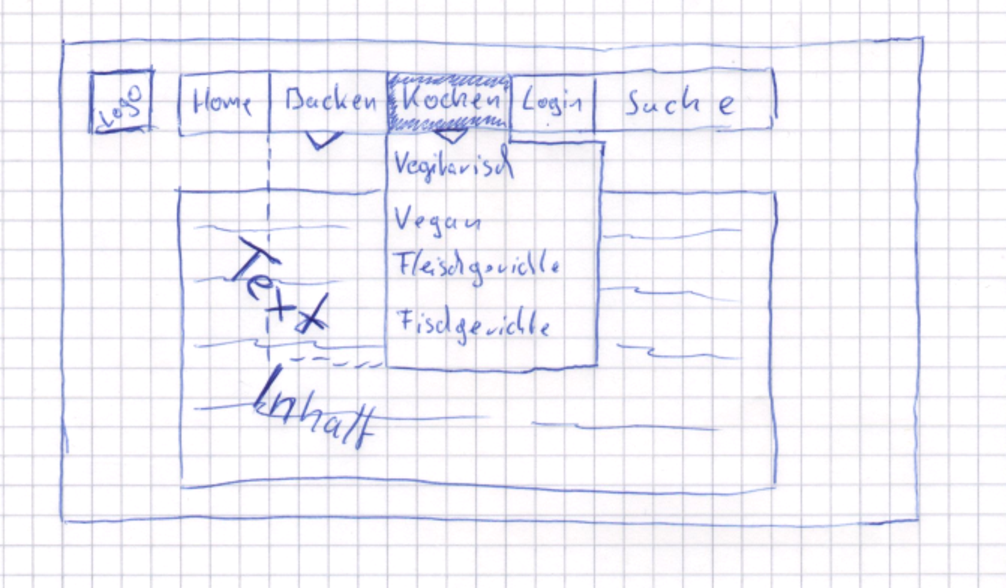
\includegraphics[scale=0.8]{Entwürfe/Chris/chris1.pdf}


\textbf{Vorteile:} \\
- einfach und übersichtlich\\
- Seite nicht überladen\\
- viel Platz für Inhalt

\textbf{Nachteile:} \\
- Menüpunkte Backen/Kochen können unübersichtlich werden bei zu vielen Unterkategorien\\
- unklar, was Login beinhaltet (welche Funktionen hat man davon?) $\to$ Hinweis auf persönliche Funktionen / Möglichkeiten

% ------------------------------------------------------------------------------------
\section*{Entwurf 2} % Chris 2

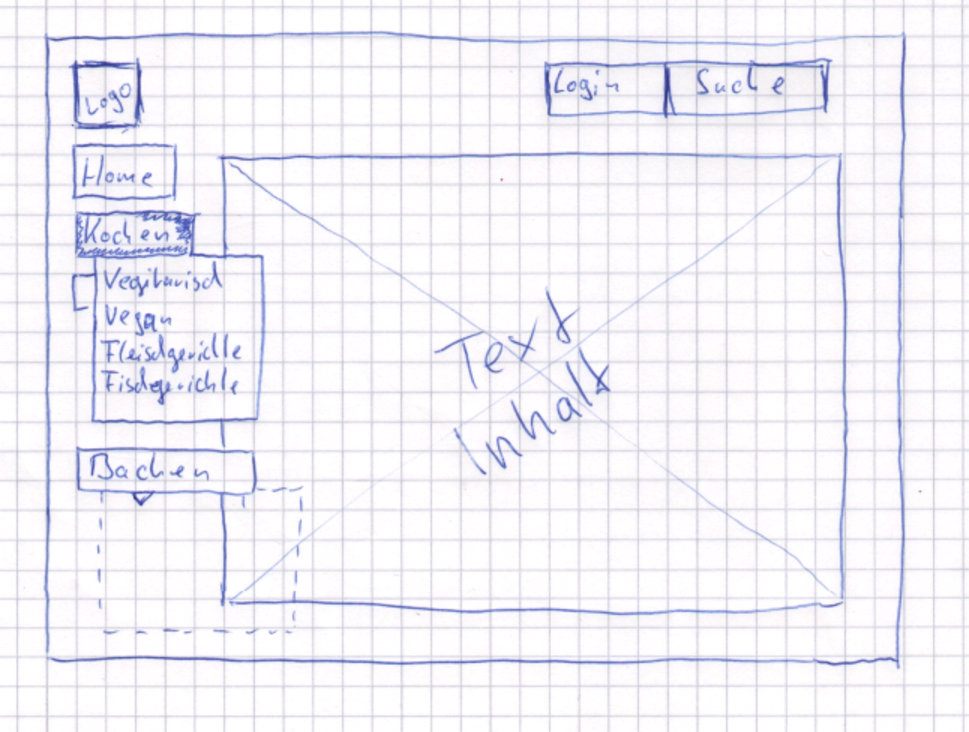
\includegraphics[scale=0.8]{Entwürfe/Chris/chris2.pdf}

\textbf{Vorteile:}\\
- klassischer Aufbau und daher intuitives Zurechtfinden möglich (Position von Login und Suche) \\
- übersichtliches Menü, das sich anpasst (Ein- und Ausklappen möglich).
-

\textbf{Nachteile:}\\
- Seitenmenü kann problematisch werden, wenn Menüpunkte zu lang sind.\\
- nicht innovativ, da es sehr oft verwendet wird.


% ------------------------------------------------------------------------------------
\section*{Entwurf 3} % Velat 1

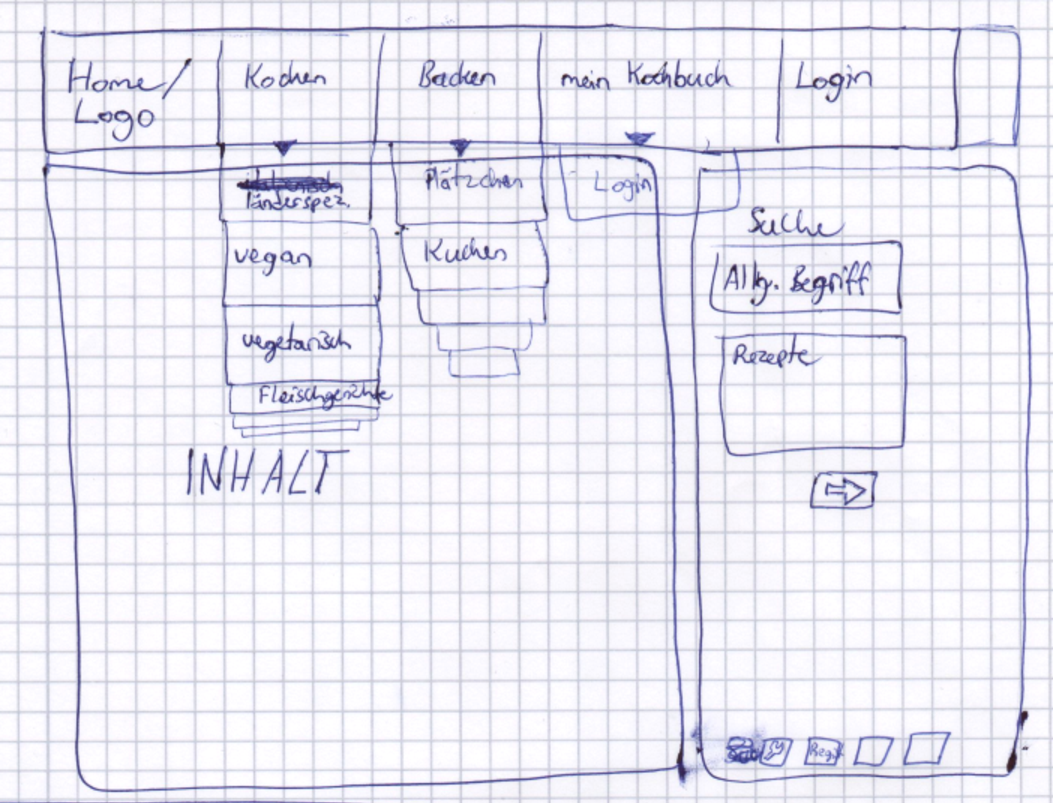
\includegraphics[scale=0.8]{Entwürfe/Velat/velat1.pdf}


\textbf{Vorteile:}\\
- es ist ersichtlich, dass es einen eigenen Kochbuchbereich gibt, für den man sich einloggen muss.\\
- innovativer Suchbereich\\
- Suchbereich als eigener Frame jederzeit sichtbar


\textbf{Nachteile:}\\
- Menüpunkte haben zu viele Unterpunkte im Dropdownmenü\\
- Suchbereich verbraucht Platz von Inhaltsseite\\
- Suchfunktion zu kompliziert

% ------------------------------------------------------------------------------------
\section*{Entwurf 4} % Velat 2

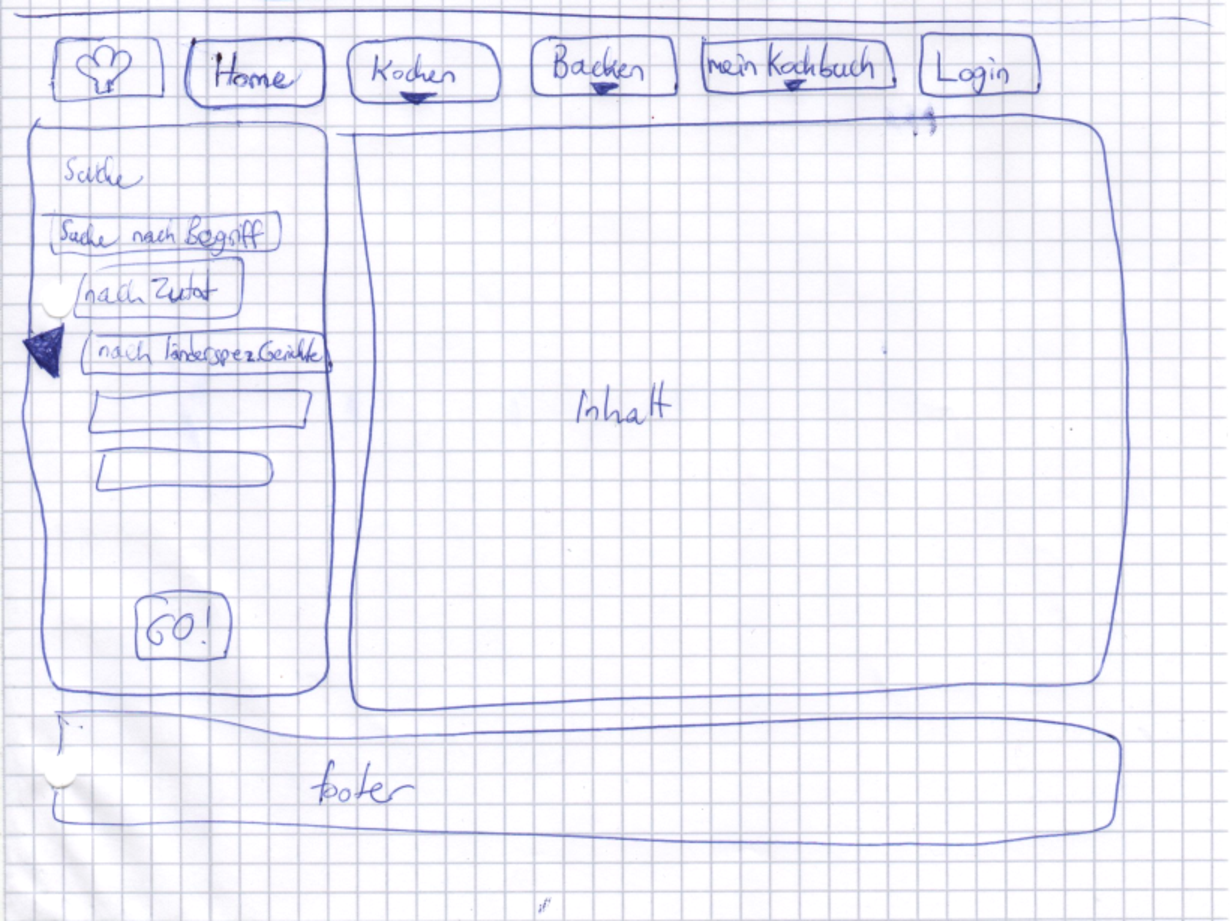
\includegraphics[scale=0.8]{Entwürfe/Velat/velat2.pdf}


\textbf{Vorteile:}\\
- seitlicher Suchbereich: Kategorien können aus- und eingeklappt werden: übersichtlich\\
- mehr Platz für Inhalt, da Suchbereich verborgen werden kann.

\textbf{Nachteile:}\\
- Im Dropdownmenü ist persönl. Bereich schon enthalten, obwohl noch nicht eingeloggt.

\newpage
% ------------------------------------------------------------------------------------
\section*{Entwurf 5} % Tamar 1

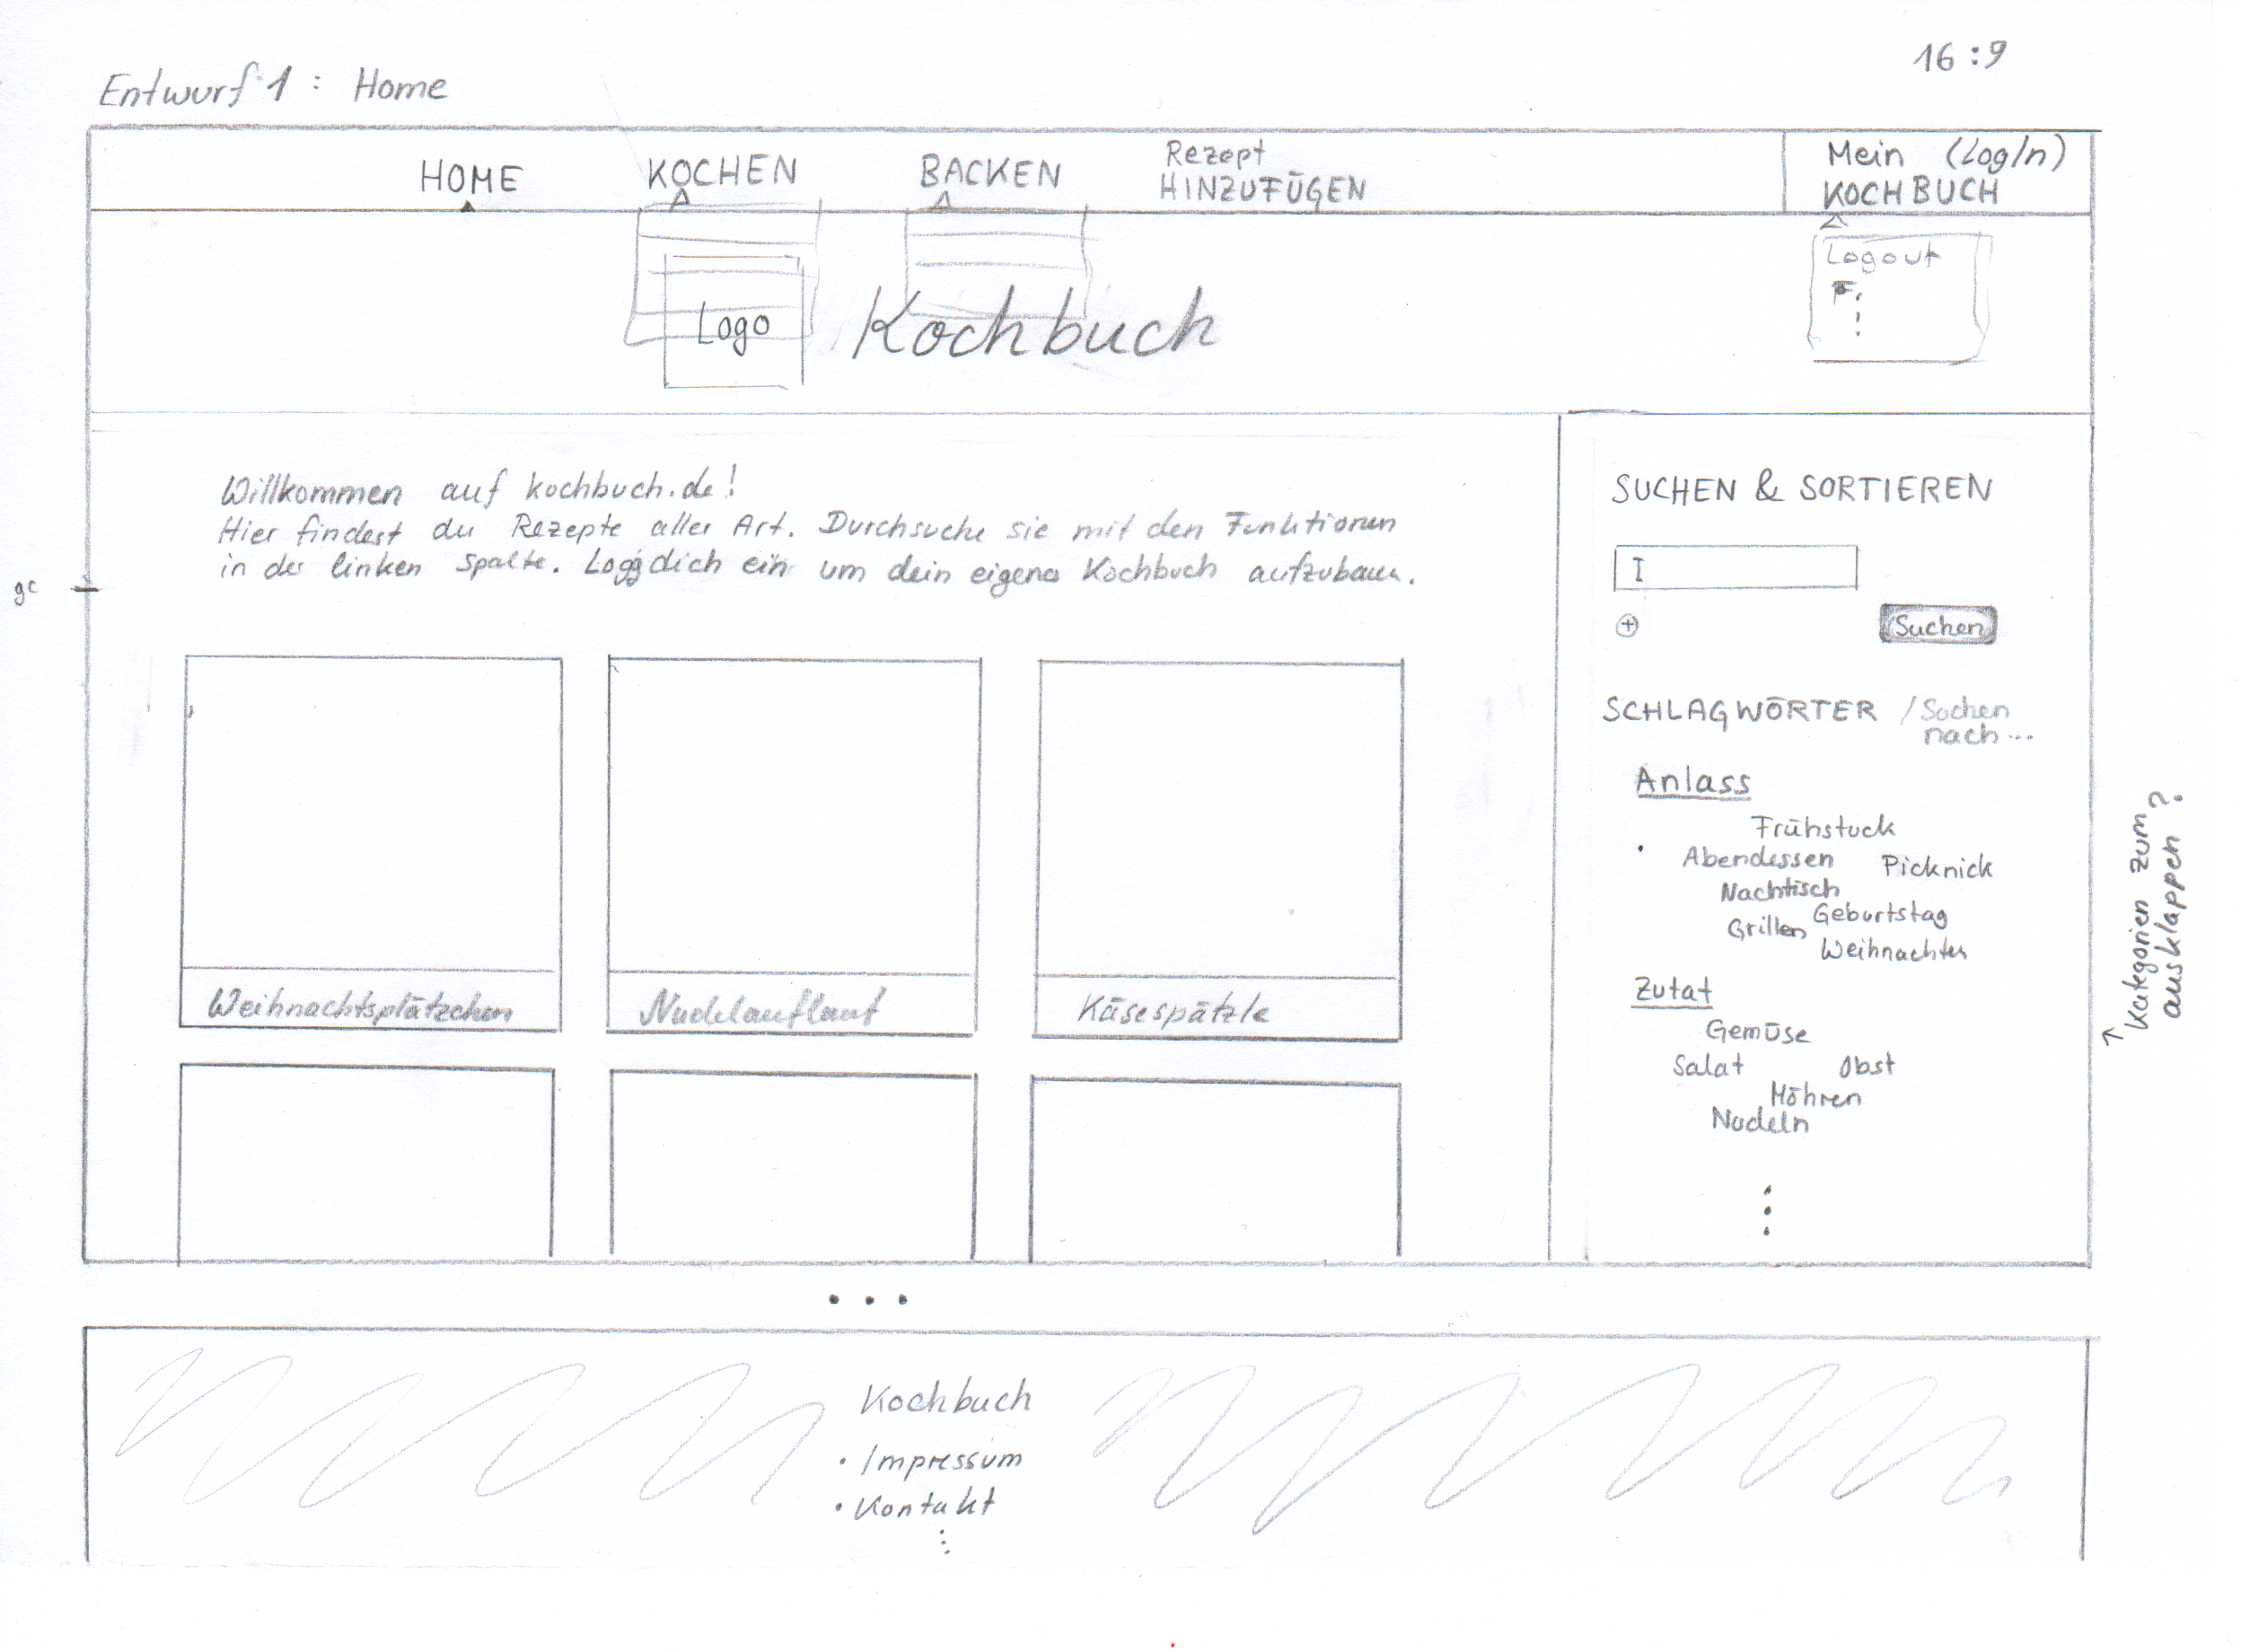
\includegraphics[scale=1]{Entwürfe/Tamar/entwurf1.1_home.png}\\
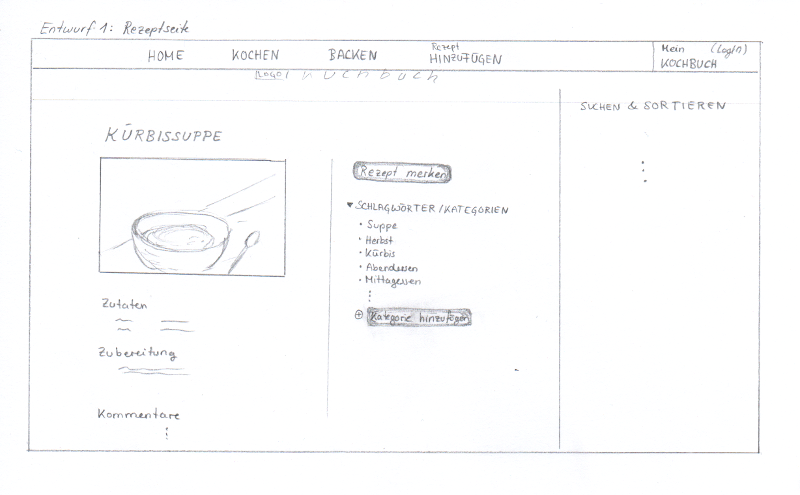
\includegraphics[scale=1]{Entwürfe/Tamar/entwurf1.2_rezeptseite.png}
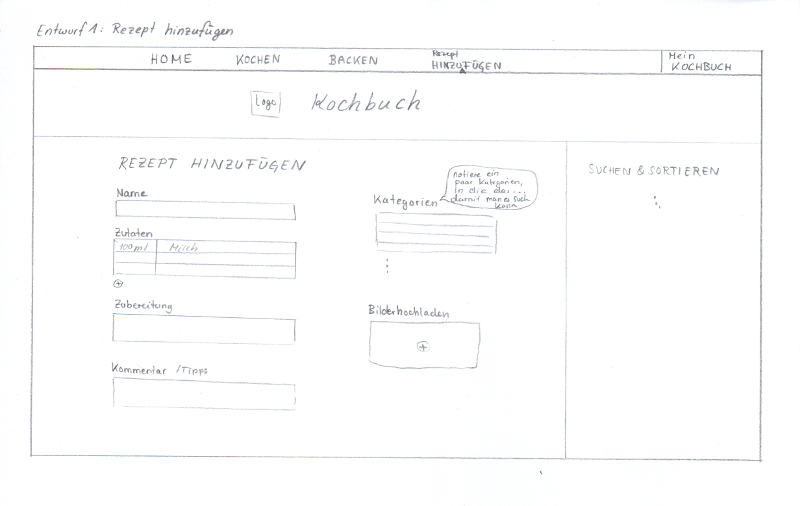
\includegraphics[scale=1]{Entwürfe/Tamar/entwurf1.3_hinzufügen.png}



\textbf{Vorteile:}\\
- klassischer Aufbau\\
- Suche jederzeit sichtbar\\
- übersichtlich

\textbf{Nachteile:}\\
- Rezept hinzufügen sollte unter mein Kochbuch kommen, da es sonst nicht in die Navigationsstruktur passt\\
- Suchfunktion verbraucht Platz\\
- auf Rezeptseite muss Rezept mehr Platz einnehmen
\newpage
% ------------------------------------------------------------------------------------
\section*{Entwurf 6} % Tamar 2

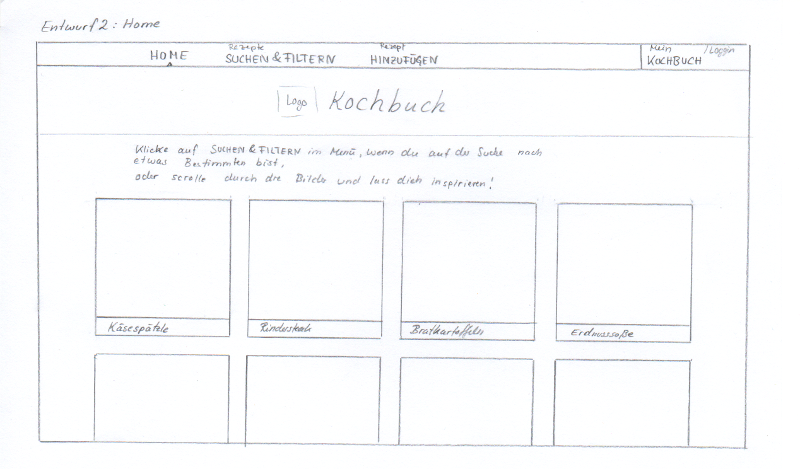
\includegraphics[scale=1]{Entwürfe/Tamar/entwurf2.1_home.png}
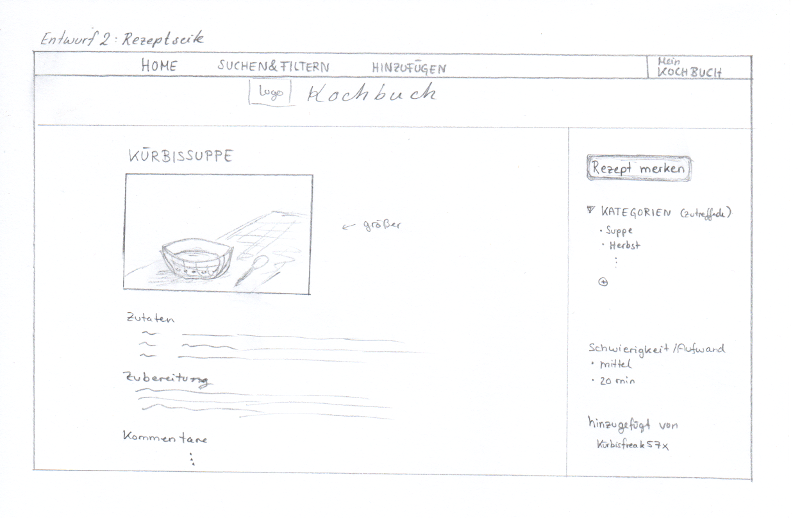
\includegraphics[scale=1]{Entwürfe/Tamar/entwurf2.2_rezeptseite.png}\\
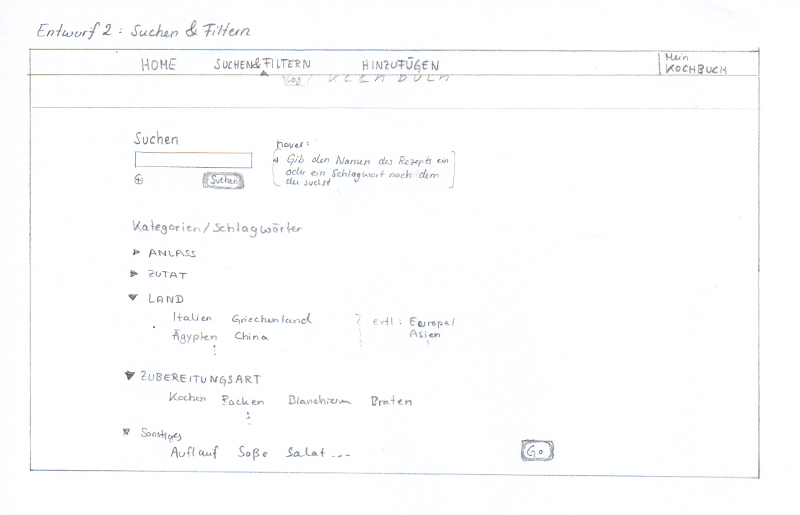
\includegraphics[scale=1]{Entwürfe/Tamar/entwurf2.3_filtern1.png}
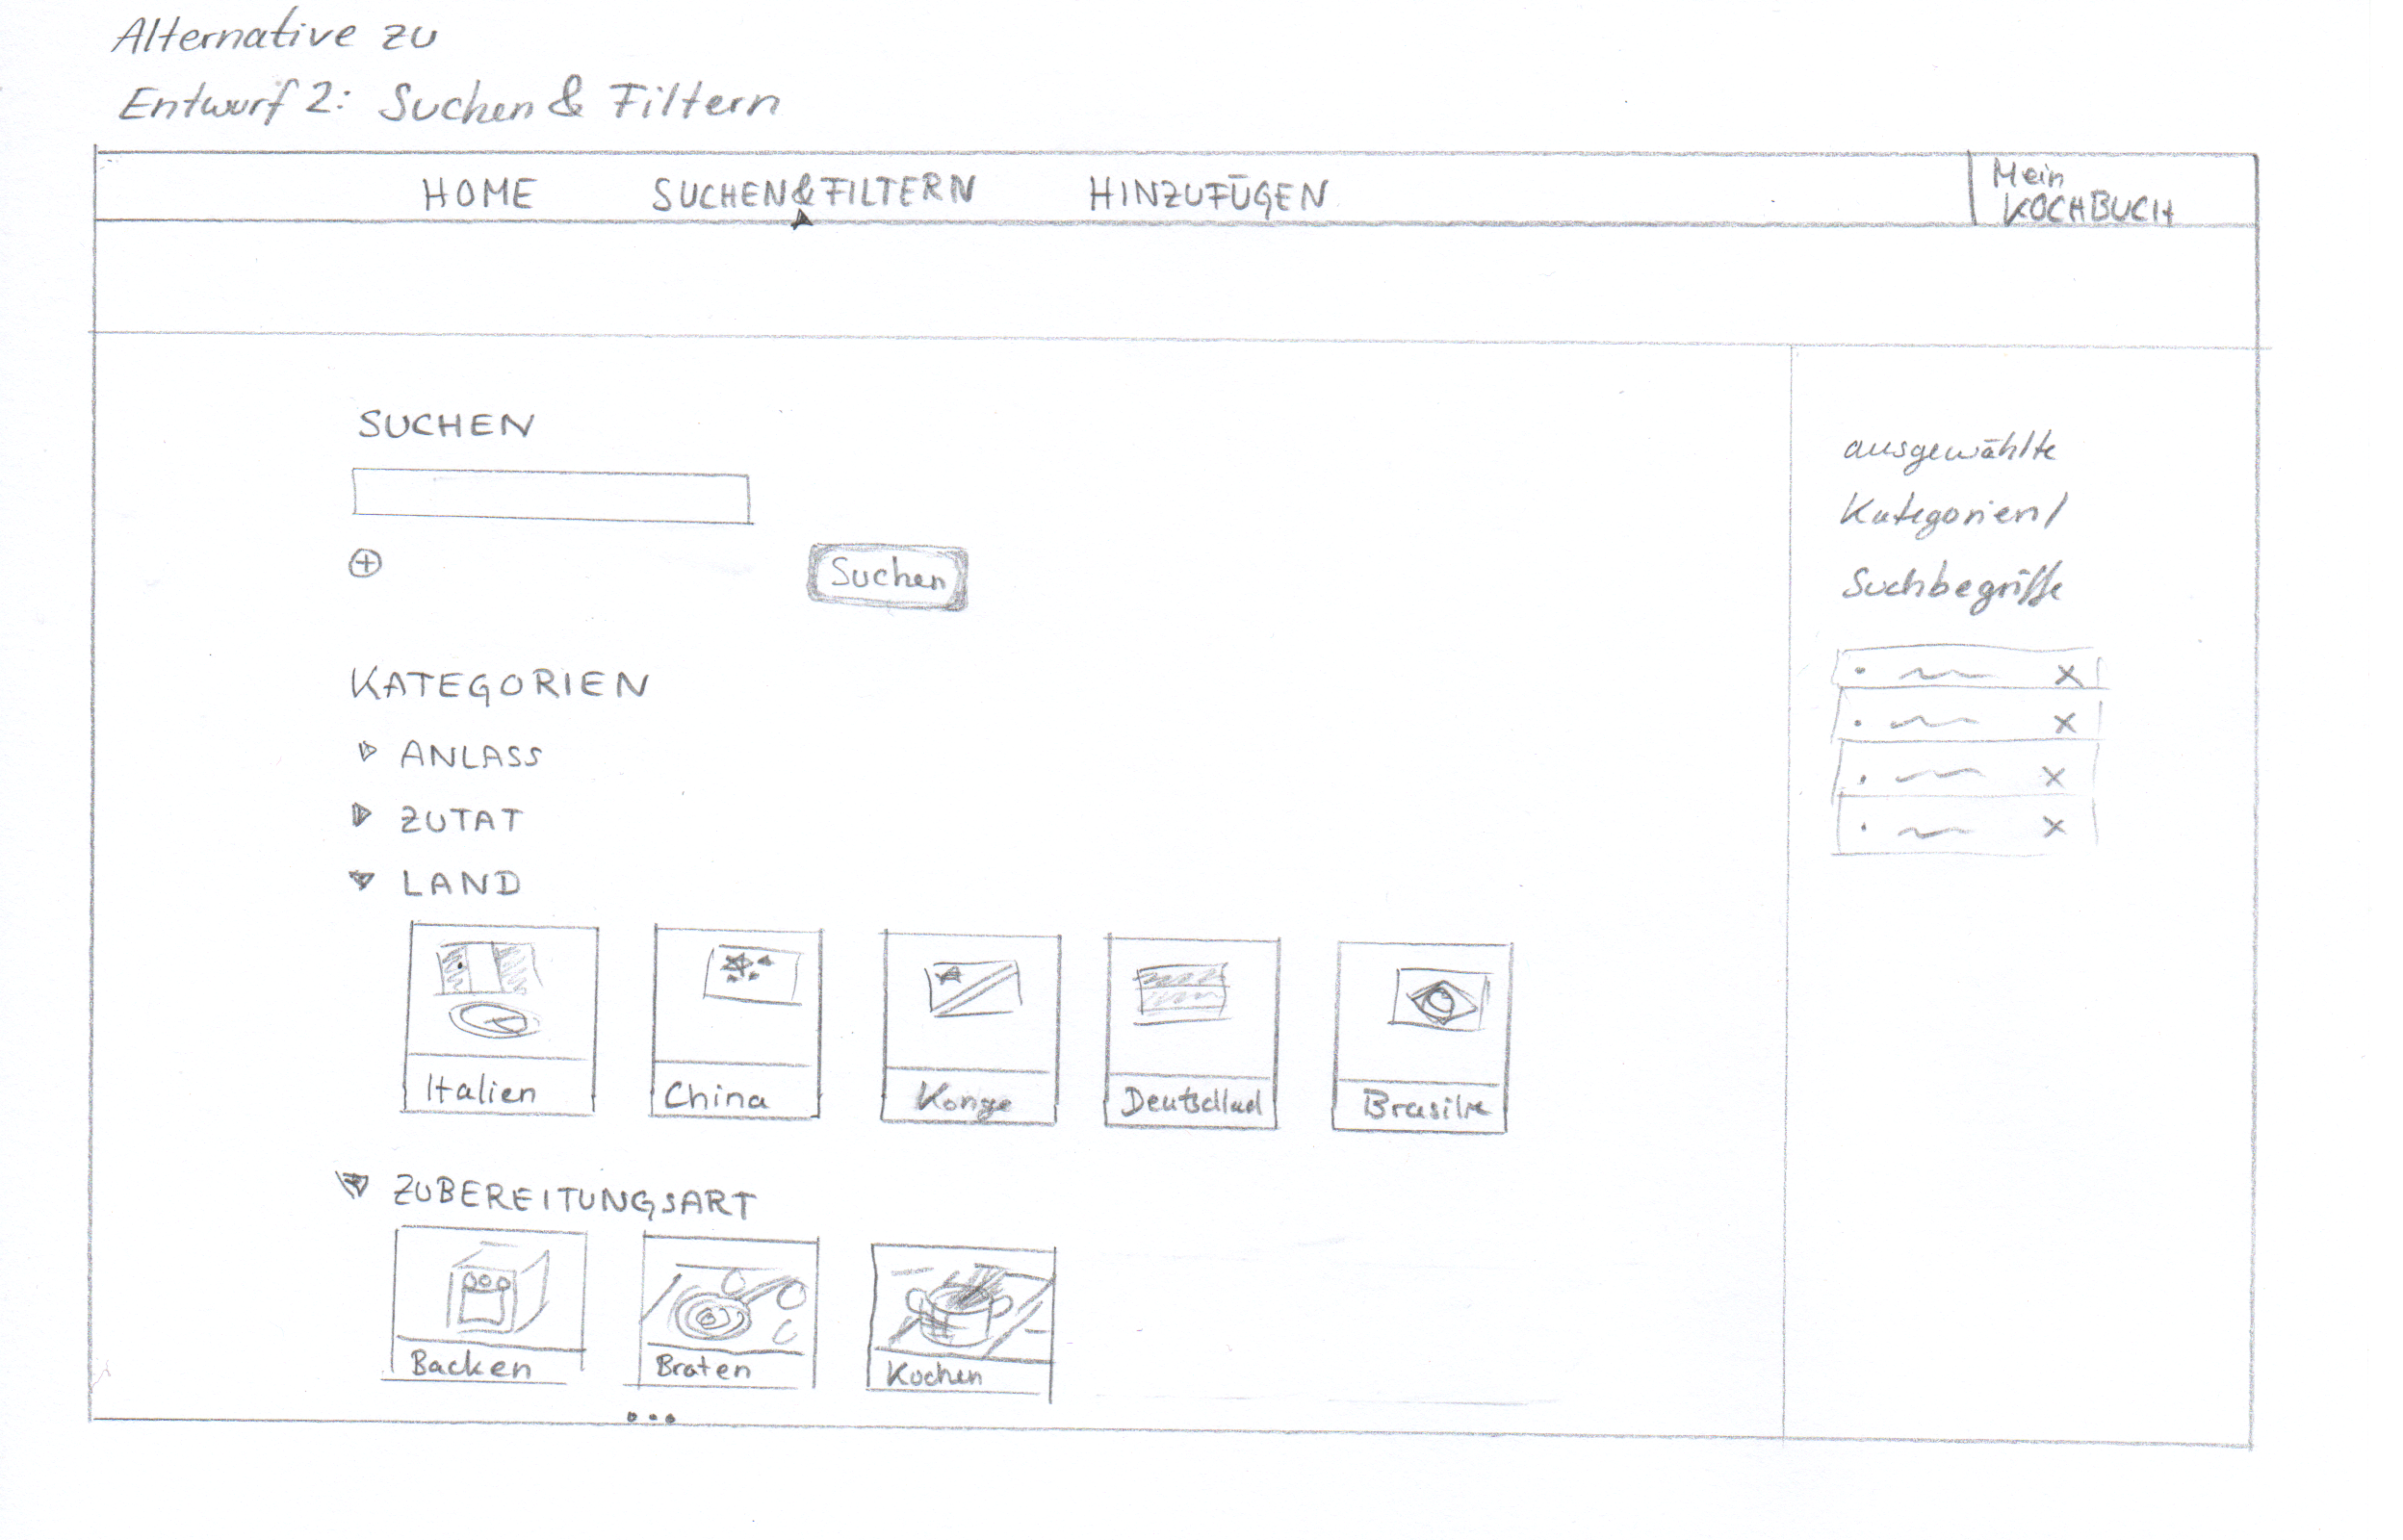
\includegraphics[scale=1]{Entwürfe/Tamar/entwurf2.3_filtern2.png}


\textbf{Vorteile:} \\
- mehr Platz\\
- aufgeräumter

\textbf{Nachteile:}\\
- Suche als eigene Seite hat Nachteil, dass man ausgewählte Kategorien nicht nebenher sieht.\\
- Suchseite zu überladen


\pagebreak
% ------------------------------------------------------------------------------------
\section*{Planung des Prototypen}

\begin{enumerate}
 \item möglichst übersichtliches, klassisches Design um intuitives Zurechtfinden zu ermöglichen (rechts oben Login)
 \item Navigation aufgespalten:
 \begin{itemize}
  \item einerseits: horizontale Navigation stellt organisatorisches dar: Meta-Navigation, wie Home und Profilverwaltung / persönlicher Bereich
  \item andererseits: Seitenmenü enthält Kategorien, nach denen Rezepte sortiert/gefiltert werden können. Für Nutzer, die genau wissen was sie wollen, gibt es die Suchleiste.
 \end{itemize}
 \item Navigation und Struktur der Webseite ist für den Nutzer ersichtlich, da auf jeder Seite Navigation an gleicher Stelle bleibt und sich eventuell dynamisch anpasst (checkboxen)
 \item Navigation nimmt nicht notwendigerweise zu viel Platz der Webseite ein, da sie eingeklappt/verborgen werden kann
 \item Damit das seitliche Menü ersichtlich bleibt, sind einzelne Kategorien (Kochen, Backen, usw.) eingeklappt. Nach Bedarf können diese ausgeklappt werden, damit Unterkategorien sichtbar sind. 
 \item Der Großteil des Seiteninhalts besteht aus Bildern von Rezepten und der dazugehörige Kochvorgang.

\end{enumerate}



\pagebreak
% ------------------------------------------------------------------------------------
% AUFGABE 4
% ------------------------------------------------------------------------------------
\section{Prototyp}


% ------------------------------------------------------------------------------------
\subsection*{Grundaufbau}

Startseite:
\begin{center}
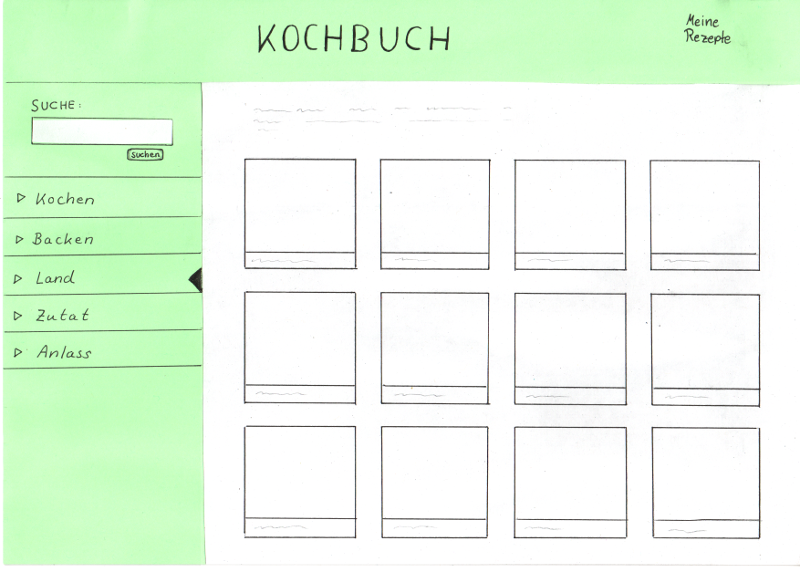
\includegraphics[scale=0.4]{Prototyp/home.png}
\end{center}

Die Startseite enthält einen kurzen Begrüßungstext mit einer kurzen Erklärung der Navigation und Bilder von verschiedenen Rezepten.\\
Rechts oben befindet sich der Menüpunkt der zum persönlichen Kochbuch bzw. Login führt.\\
Auf der linken Seite gibt es die Möglichkeit, die Rezepte nach Belieben zu filtern. Entweder nach Suchbegriffen oder nach verschiedenen Kategorien, die auf dem Prototypen in einer Auswahl dargestellt sind.

\pagebreak
Rezeptseite:
\begin{center}
\includegraphics[scale=0.4]{Prototyp/plätzchenrezeptseite.png}
\end{center}

Eine Rezeptseite enthält ein Bild, Zutaten, Zubereitung und Kommentare zu einem Rezept. In dem Bereich auf der rechten Seite befindet sich der Button, um das Rezept zu speichern. Ist man nicht eingeloggt, wird man aufgefordert, sich einzuloggen. 
Außerdem befinden sich auf der Seite Informationen zum Aufwand des Gerichtes und die Kategorie, in der es sich befindet. 

\pagebreak
% ------------------------------------------------------------------------------------
\subsection*{Funktionalität der Navigation}

Einklappen der Seitennavigation:
\begin{center}
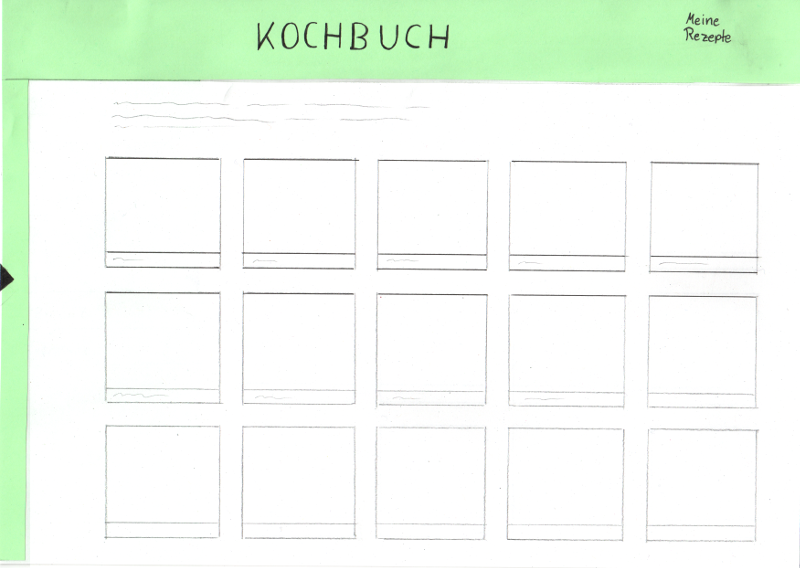
\includegraphics[scale=0.4]{Prototyp/home_menuhidden.png}
\end{center}

Die Seitennavigation kann durch Betätigung des Pfeiles auf der linken Seite ein- bzw. ausgeklappt werden. 

horizontales Menü: meine Rezepte
\begin{center}
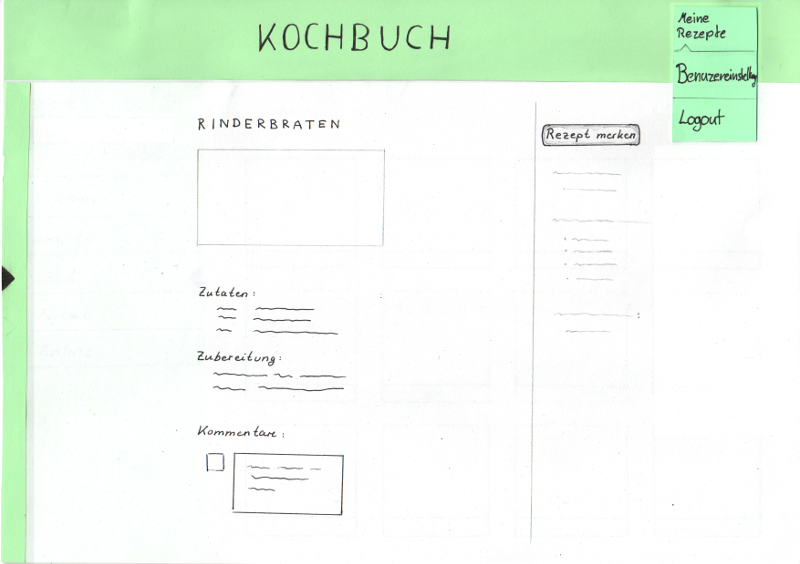
\includegraphics[scale=0.4]{Prototyp/menu_eigeneRezepte_menuhidden.png}
\end{center}


Die einzelnen Menüpunkte sind durch Anklicken des Pfeiles aufklappbar:

Menü: Kochen
\begin{center}
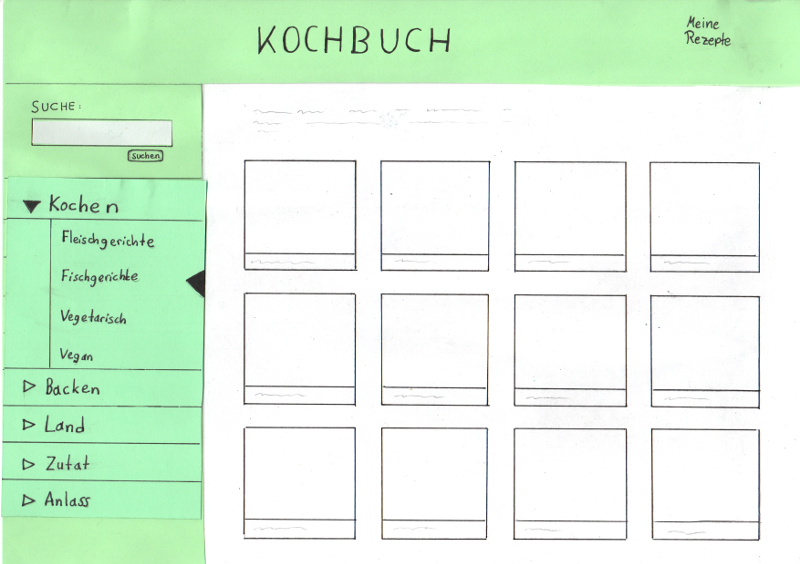
\includegraphics[scale=0.4]{Prototyp/menu_kochen.png}
\end{center}

Menü: Backen
\begin{center}
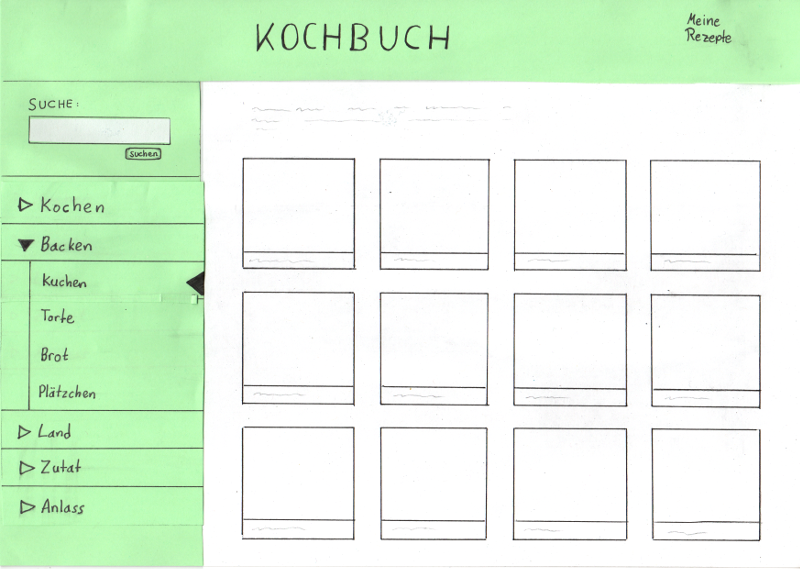
\includegraphics[scale=0.4]{Prototyp/menu_backen.png}
\end{center}
\newpage
Menü: Zutat
\begin{center}
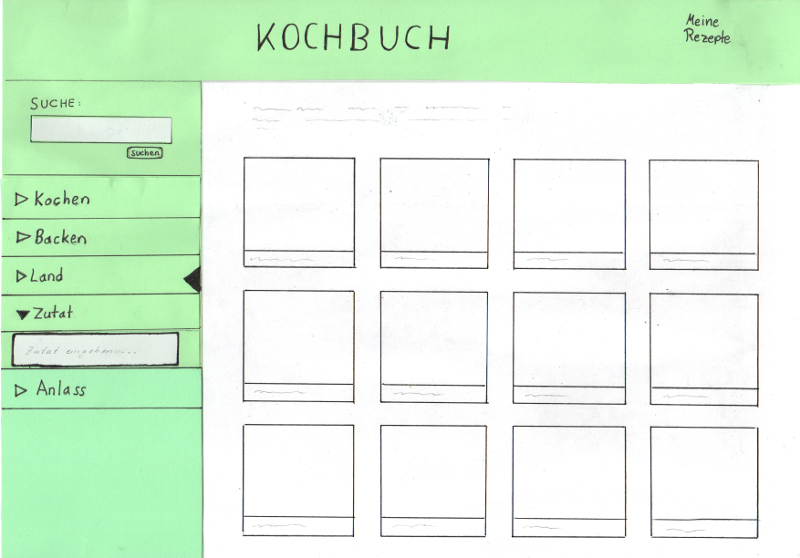
\includegraphics[scale=0.4]{Prototyp/menu_zutat.png}
\end{center}

\pagebreak
% ------------------------------------------------------------------------------------
\subsection*{Szenarien}

\subsubsection*{Szenario 1: Max will Plätzchen backen}

Er verwendet die Suchfunktion, gibt "Plätzchen" ein und erhält Plätzchenrezepte.
\begin{center}
\includegraphics[scale=0.4]{Prototyp/plätzchensuche.png}
\end{center}

Er wählt ein Rezept aus und wird auf die entsprechende Rezeptseite gebracht.
\begin{center}
\includegraphics[scale=0.4]{Prototyp/plätzchenrezeptseite.png}
\end{center}


\subsubsection*{Szenario 2: Karl hat nur bestimmte Zutaten da}

Er wählt im Seitenmenü "Zutat" aus...
\begin{center}
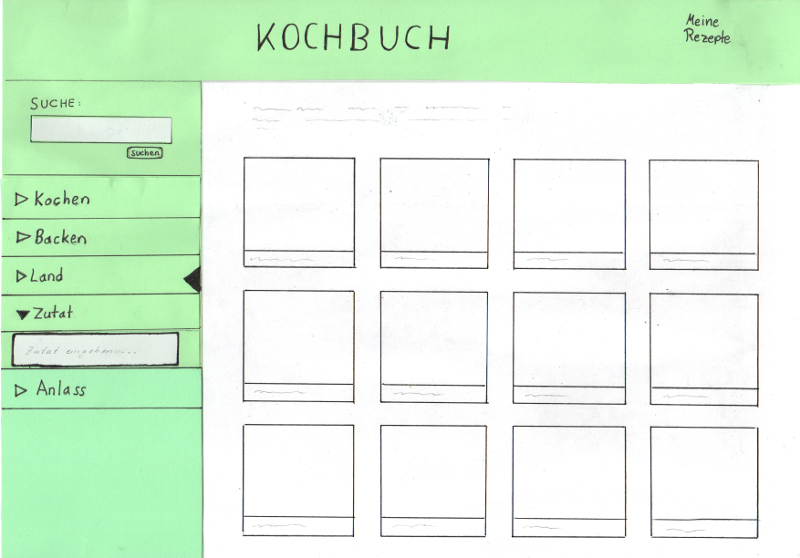
\includegraphics[scale=0.4]{Prototyp/menu_zutat.png}
\end{center}

... und gibt die Zutaten ein, die ihm zur Verfügung stehen: Nudeln, Hackfleisch und Tomaten
\begin{center}
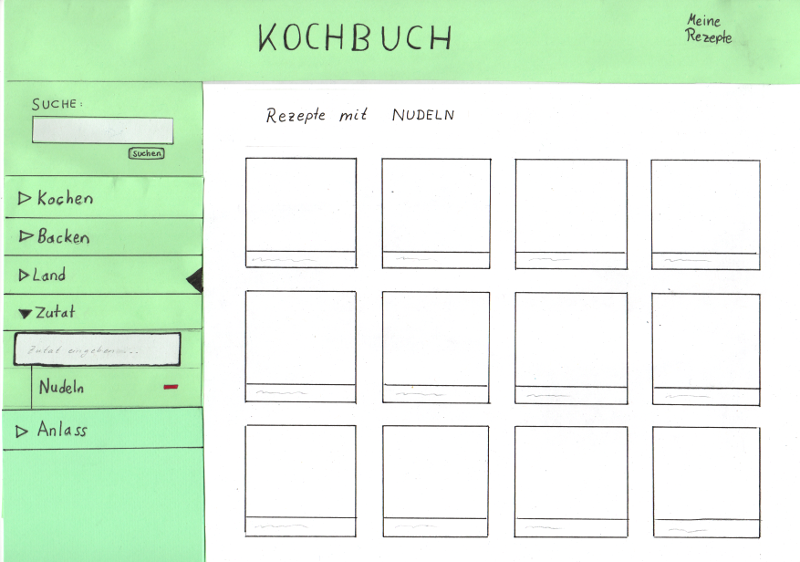
\includegraphics[scale=0.4]{Prototyp/menu_zutat_nudeln.png}\\[1em]
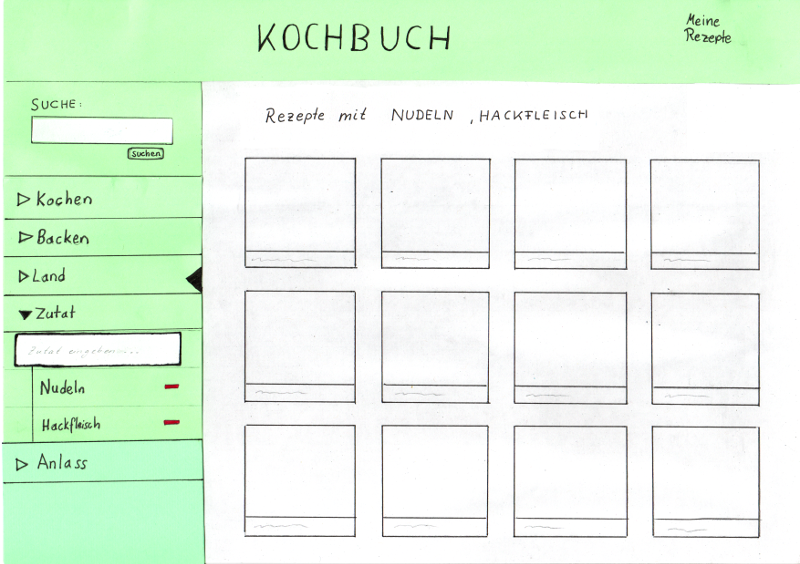
\includegraphics[scale=0.4]{Prototyp/menu_zutat_nudelnhackfleisch.png}\\[1em]
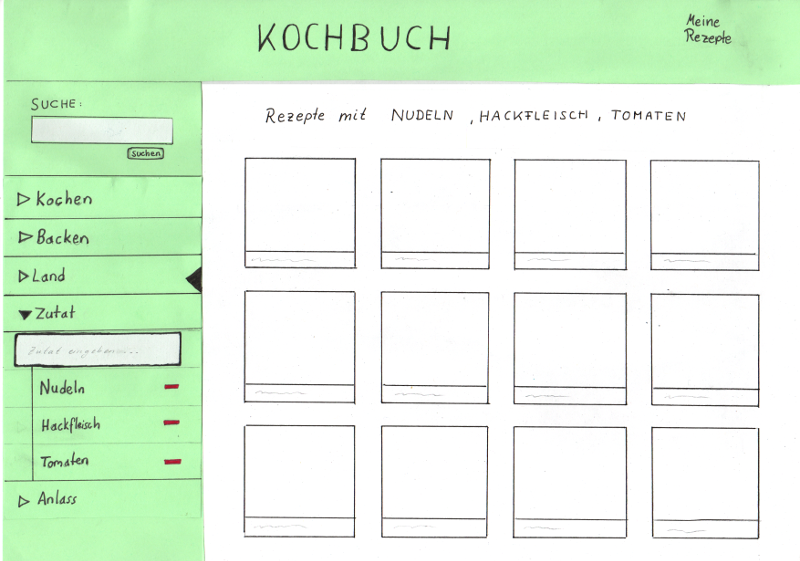
\includegraphics[scale=0.4]{Prototyp/menu_zutat_nudelnhackfleischtomate.png}
\end{center}
Er bekommt eine Auswahl von Rezepten, die zu seinen Zutaten passen.

\pagebreak
\subsubsection*{Szenario 3: Anna lässt sich inspirieren}

Anna klappt das Seitenmenü ein, um auf der gesamten Breite die Bilder der Rezepte betrachten zu können.
\begin{center}
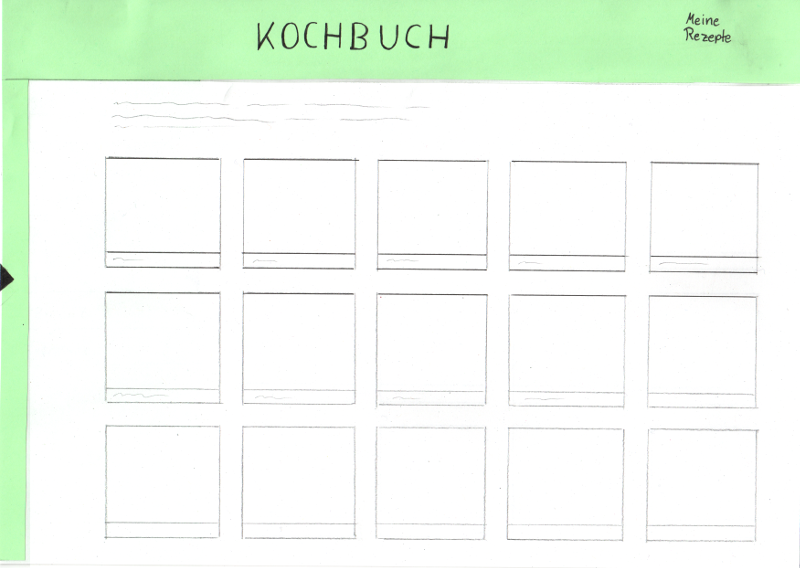
\includegraphics[scale=0.4]{Prototyp/home_menuhidden.png}
\end{center}

Sie scrollt durch die Bilder und sieht sich ein bestimmtes Rezept an.
\begin{center}
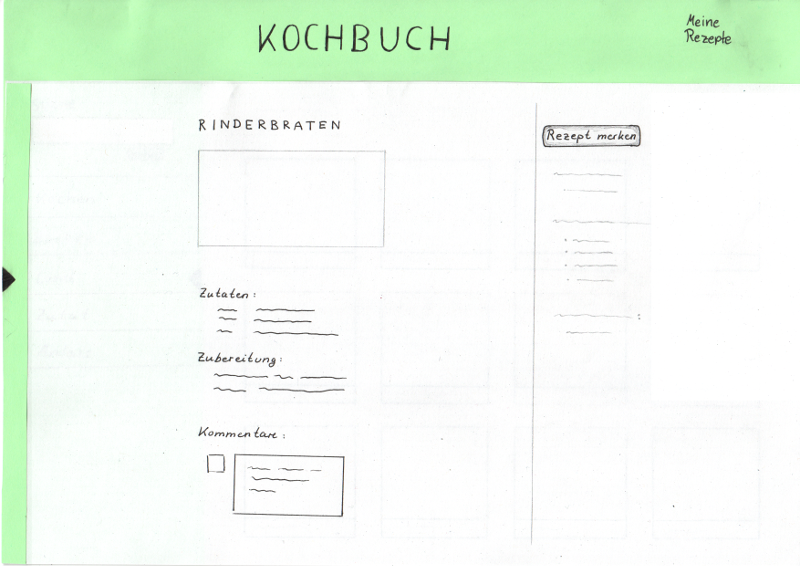
\includegraphics[scale=0.4]{Prototyp/rezeptseite_menuhidden.png}
\end{center}

Sie klickt auf "Rezept merken" und sieht sich dann unter "meine Rezepte" ihre bisher gespeicherten Rezepte an.
\begin{center}
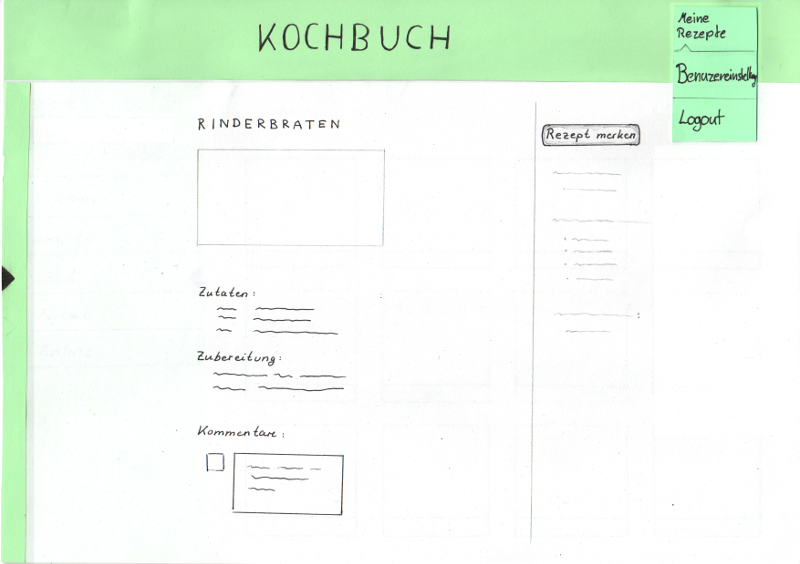
\includegraphics[scale=0.4]{Prototyp/menu_eigeneRezepte_menuhidden.png}\\[1em]
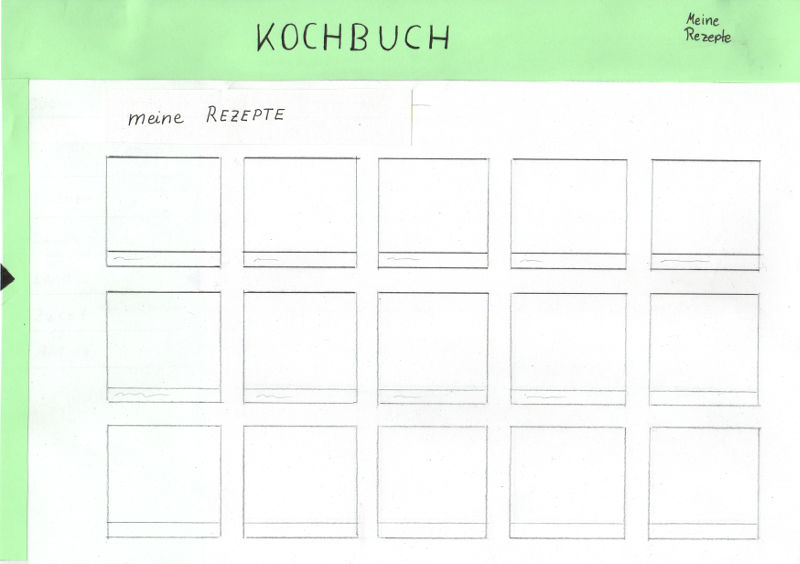
\includegraphics[scale=0.4]{Prototyp/meineRezepte_menuhidden.png}
\end{center}



% ------------------------------------------------------------------------------------
% AUFGABE 5
% ------------------------------------------------------------------------------------
%\section*{Präsentation}
\stepcounter{section}

% ------------------------------------------------------------------------------------
% AUFGABE 6
% ------------------------------------------------------------------------------------
\section{Heuristische Evaluation}

% ------------------------------------------------------------------------------------
% AUFGABE 7
% ------------------------------------------------------------------------------------
%\section{Umsetzung}
\stepcounter{section}

% ------------------------------------------------------------------------------------
% AUFGABE 8
% ------------------------------------------------------------------------------------
\section{Prüfung der Barrierefreiheit}

% ------------------------------------------------------------------------------------
% AUFGABE 9
% ------------------------------------------------------------------------------------
\section{Nutzertest}

% ------------------------------------------------------------------------------------
% AUFGABE 10
% ------------------------------------------------------------------------------------
\section{Projektabschluss}



\pagebreak
% ------------------------------------------------------------------------------------
% Anhang
% ------------------------------------------------------------------------------------
\pagenumbering{Roman}

\begin{appendix}
\section{Protokolle der Nutzertests}
%\addcontentsline{toc}{section}{Anhang}

\subsection*{Chris}
\subsection*{Velat}
\subsection*{Tamar}

\end{appendix}




\end{document}



